\section{Experimental results}

% \subsection{训练情况}

训练时验证集准确率的收敛情况如图 \ref{fig:val} 所示。由图可见,CNN 的收敛速度要比 RNN 要快,但是单个批次的训练时间 CNN 会更长一些。在 CNN 中,ResNet 的最终正确率会更高一些。将 CNN 与 RNN 结合的网络最终验证集正确率会比两者单独都要高一些。

\begin{figure}[ht]
    \centering
    \subfigure[CNN]{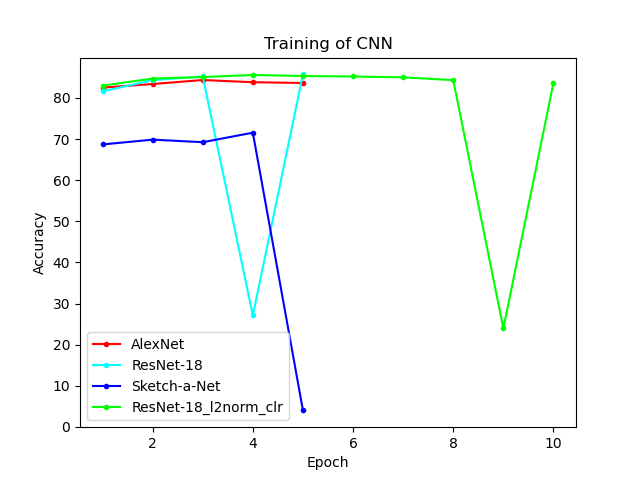
\includegraphics[width=0.3\textwidth]{img/cnn}}
    \subfigure[RNN]{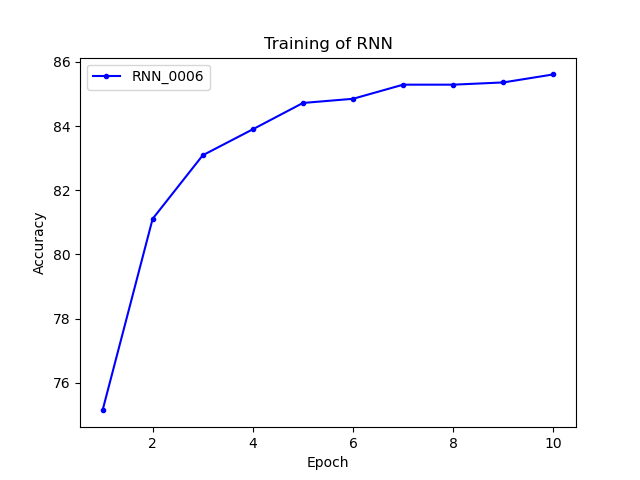
\includegraphics[width=0.3\textwidth]{img/rnn}}
    \subfigure[CNN+RNN]{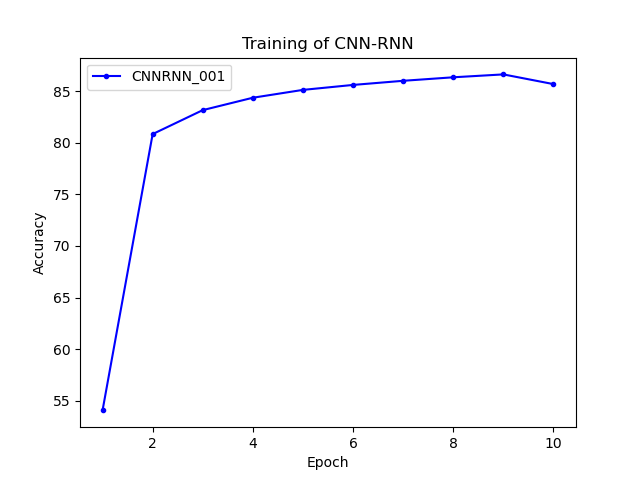
\includegraphics[width=0.3\textwidth]{img/cnnrnn.png}}
    \caption{验证集收敛情况}
    \label{fig:val}
\end{figure}

最后将最佳验证准确率对应的网络在 25 个类别所有的测试集进行测试,结果如表 \ref{tab1} 所示。


\begin{table}[H]
\begin{minipage}{0.4\textwidth}
\caption{每一类模型最佳的测试准确率}\label{tab1}
\centering
\begin{tabular}{cc}
\toprule
模型 & 测试准确率 \\
\midrule
Sketch-a-Net & 0.6948\\
AlexNet & 0.8462\\
ResNet18 & 0.8557\\
BiLSTM & 0.8561\\
CNN+RNN & \textbf{0.8567}\\
\bottomrule
\end{tabular}
\end{minipage}
\begin{minipage}{0.55\textwidth}
\centering
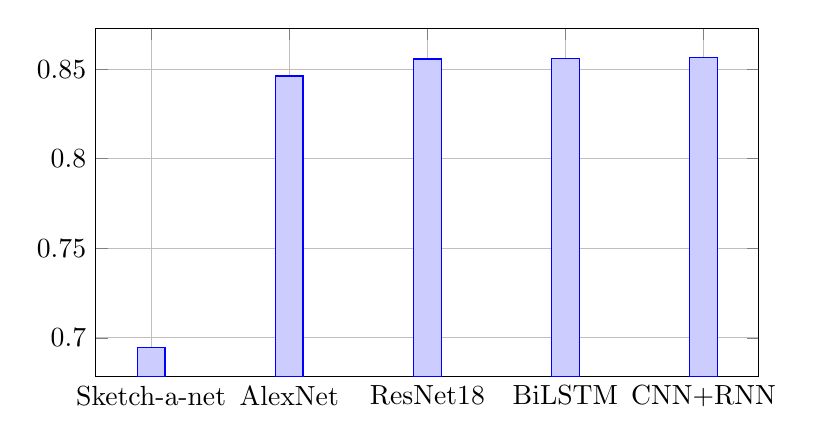
\begin{tikzpicture}
\begin{axis}[grid={major},
symbolic x coords={Sketch-a-net,AlexNet,ResNet18,BiLSTM,CNN+RNN}, xtick=data,
width=10cm,height=6cm,]
 \addplot+ [ybar,no markers,fill=blue!20,] table[row sep=crcr,x=model,y=acc,] {model acc\\Sketch-a-net 0.6948\\AlexNet 0.8462\\ResNet18 0.8557\\BiLSTM 0.8561\\CNN+RNN 0.8567\\};
\end{axis}
\end{tikzpicture}

\captionof{figure}{测试准确率统计图}
\end{minipage}
\end{table}

